\documentclass[11pt]{article}
\usepackage[margin=0.95in]{geometry}
\usepackage{graphicx}
\usepackage{subcaption}
\usepackage{booktabs}
\usepackage{hyperref}
\usepackage{url}
\usepackage{enumitem}
\setlist{nosep}
\usepackage[skip=4pt]{caption}
\usepackage{titlesec}
\titlespacing*{\section}{0pt}{9pt}{4pt}
\titlespacing*{\subsection}{0pt}{7pt}{3pt}

\title{CSE 398/498 Lab 1 Report:\\Object Detection with YOLOv11 and YOLOE}
\author{Hengde Dai \\ \texttt{hed424@lehigh.edu}}
\date{September 2, 2026}

\begin{document}

\maketitle

\section{Introduction}

Lab 1 consists of three experiments. First, I ran a pretrained YOLOv11 model on my laptop webcam and tested how well it recognizes everyday objects. Second, I fine-tuned YOLOv11 on a small custom dataset that targets an object the pretrained model could not recognize, and I repeated the webcam experiment to check whether fine-tuning helps. Third, I followed the assigned Colab notebook on YOLOE to learn open-set object detection. The report explains how YOLOv11 works, what I learned from fine-tuning, what open-set object detection is, and how the YOLOE architecture supports it.

All code, the dataset, the trained weights, and the executed notebooks are collected in my GitHub repository.\footnote{\url{https://github.com/DylanDai63/cse498-lab1}} The webcam experiments ran locally (Windows 11, RTX 3070 Ti, PyTorch 2.5.1 with CUDA 12.1, \texttt{ultralytics} 8.4.135). Training and the YOLOE notebook ran on a Colab T4 GPU with \texttt{ultralytics} 8.3.40.

\section{Experiment 1: Pretrained YOLOv11 on a Webcam}

\subsection{Setup}

I cloned the assigned \texttt{webcam-object-recognition} repository and vendored it into my submission repository. The script loads COCO-pretrained \texttt{yolo11n.pt}, reads webcam frames in a loop, runs detection with a 0.5 confidence threshold, and draws labeled boxes. My only change, documented in the commit history, was disabling per-frame console logging, which degraded the editor over long runs.

\subsection{Results}

I held nine household objects in front of the camera one at a time. Table~\ref{tab:step1} summarizes the outcomes, and Figure~\ref{fig:step1} shows one success and the failure case that motivated Experiment 2.

\begin{table}[h]
\centering
\small
\begin{tabular}{llll}
\toprule
Object & Prediction & Confidence & Outcome \\
\midrule
Water bottle & bottle & 0.91 & correct \\
Couch & couch & 0.85 & correct \\
Scissors & scissors & 0.80 & correct \\
Book & book & 0.78 & correct \\
Cell phone & cell phone & 0.78 & correct \\
Game controller & remote & 0.82 & near miss (no controller class in COCO) \\
\midrule
Vine tomatoes & apple & 0.52--0.62 & misclassified \\
Toilet paper (upright) & cup & 0.59 & misclassified \\
Toilet paper (on side) & toilet & 0.53 & misclassified \\
\bottomrule
\end{tabular}
\caption{Pretrained YOLOv11n webcam results. Screenshots for every row are archived in \texttt{step1-webcam-yolov11/results-pretrained/}.}
\label{tab:step1}
\end{table}

\begin{figure}[h]
\centering
\begin{subfigure}{0.38\textwidth}
  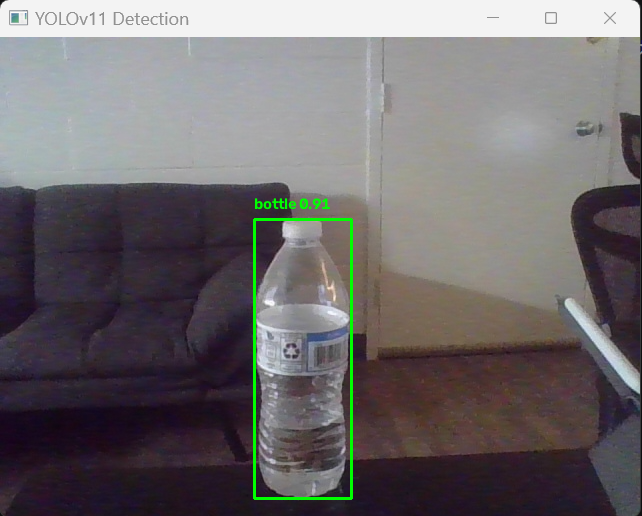
\includegraphics[width=\textwidth]{figures/step1_ok_bottle.png}
  \caption{Correct: bottle, 0.91.}
\end{subfigure}
\hfill
\begin{subfigure}{0.38\textwidth}
  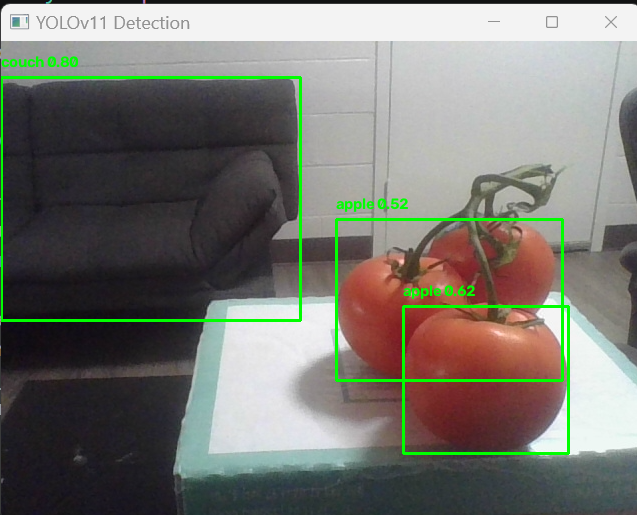
\includegraphics[width=\textwidth]{figures/before_tomato_as_apple.png}
  \caption{Failure: tomatoes labeled apple, 0.52--0.62.}
\end{subfigure}
\caption{Pretrained YOLOv11n on the webcam.}
\label{fig:step1}
\end{figure}

The failures follow one pattern. COCO has 80 classes, and none of the failed objects is among them. The model therefore mapped each object to the nearest class it knows: tomatoes to apple, a paper roll to cup or toilet. The model cannot output a word it was never trained on. That observation sets up both remaining experiments: fine-tuning adds a missing class by retraining, and open-set detection removes the fixed class list altogether.

\section{How YOLOv11 Works}

YOLO stands for ``You Only Look Once.'' The model treats detection as a single regression problem: one forward pass of a convolutional network over the full image directly outputs box coordinates, a confidence score, and class scores. Two-stage detectors such as R-CNN first propose candidate regions and then classify each region. The single-stage design trades a small amount of accuracy for much higher speed, which is why the webcam demo runs in real time (about 7~ms per frame on my GPU).

Conceptually, the image is divided into an $S \times S$ grid. Each cell predicts a fixed number of boxes, each with coordinates $(x, y, w, h)$ and a confidence score, together with class scores. The cell containing an object's center is responsible for that object. During training, only the predicted box with the highest IoU against the ground truth is assigned to it. At inference time, many overlapping boxes survive, so non-maximum suppression (NMS) keeps the highest-confidence box and discards neighbors whose IoU exceeds a threshold.

YOLOv11 keeps the three-part structure of its predecessors: a backbone extracts features, a neck fuses features across scales, and a head outputs boxes and scores. According to the course slides, the version-specific changes include the C3k2 block, which replaces C2f in the backbone and captures multi-scale spatial detail at lower cost; the C2PSA module, which adds partial spatial attention so the network focuses on informative regions; and an optimized head in which the classification and regression branches share representation weights to cut inference latency. The result is higher COCO accuracy with fewer parameters than YOLOv8. I used the nano variant \texttt{yolo11n} (2.6M parameters) throughout the lab so that Experiments 1 and 2 stay directly comparable.

\section{Experiment 2: Fine-Tuning YOLOv11}

\subsection{Dataset}

The assignment suggested a Kaggle grocery dataset as a possible source. I downloaded it and found that it contains only a CSV of product listings, without images or bounding boxes. The instructor's revised instructions confirmed the issue and asked for a dataset with bounding-box labels, unseen classes, and YOLO format. I therefore built the dataset myself from Google Open Images, which provides human-verified box annotations.

I chose \texttt{tomato} as the target class. I verified programmatically that neither ``tomato'' nor ``toilet paper'' appears in the 80 COCO class names, so both qualify as unseen classes. The final dataset contains 50 hand-reviewed images with 99 boxes, split 42/8 into train and validation, resized to 640~px, with labels converted to YOLO format. Reaching that final set took three iterations, and each one taught me something concrete:

\begin{enumerate}
  \item A two-class draft (tomato and toilet paper) trained to mAP50 of 0.59 on tomato but only 0.01 on toilet paper. Open Images contains few usable toilet-paper images, and a class with roughly 12 training images failed to learn.
  \item A 50-image random sample of tomato reached mAP50 of 0.66, but every detection stayed below a 0.25 confidence threshold. Open Images labels anything tomato-related as ``Tomato,'' including sauces, slices, and unripe fruit, and one image showed persimmons. The noisy positives appear to have diluted the signal.
  \item I then ranked candidates by box size, reviewed about 200 images by hand across three Open Images splits, and kept 50 clean photos of whole, mostly red tomatoes. I excluded dense piles whose annotations do not cover every visible tomato, since unlabeled objects would count as background during training.
\end{enumerate}

\begin{figure}[h]
\centering
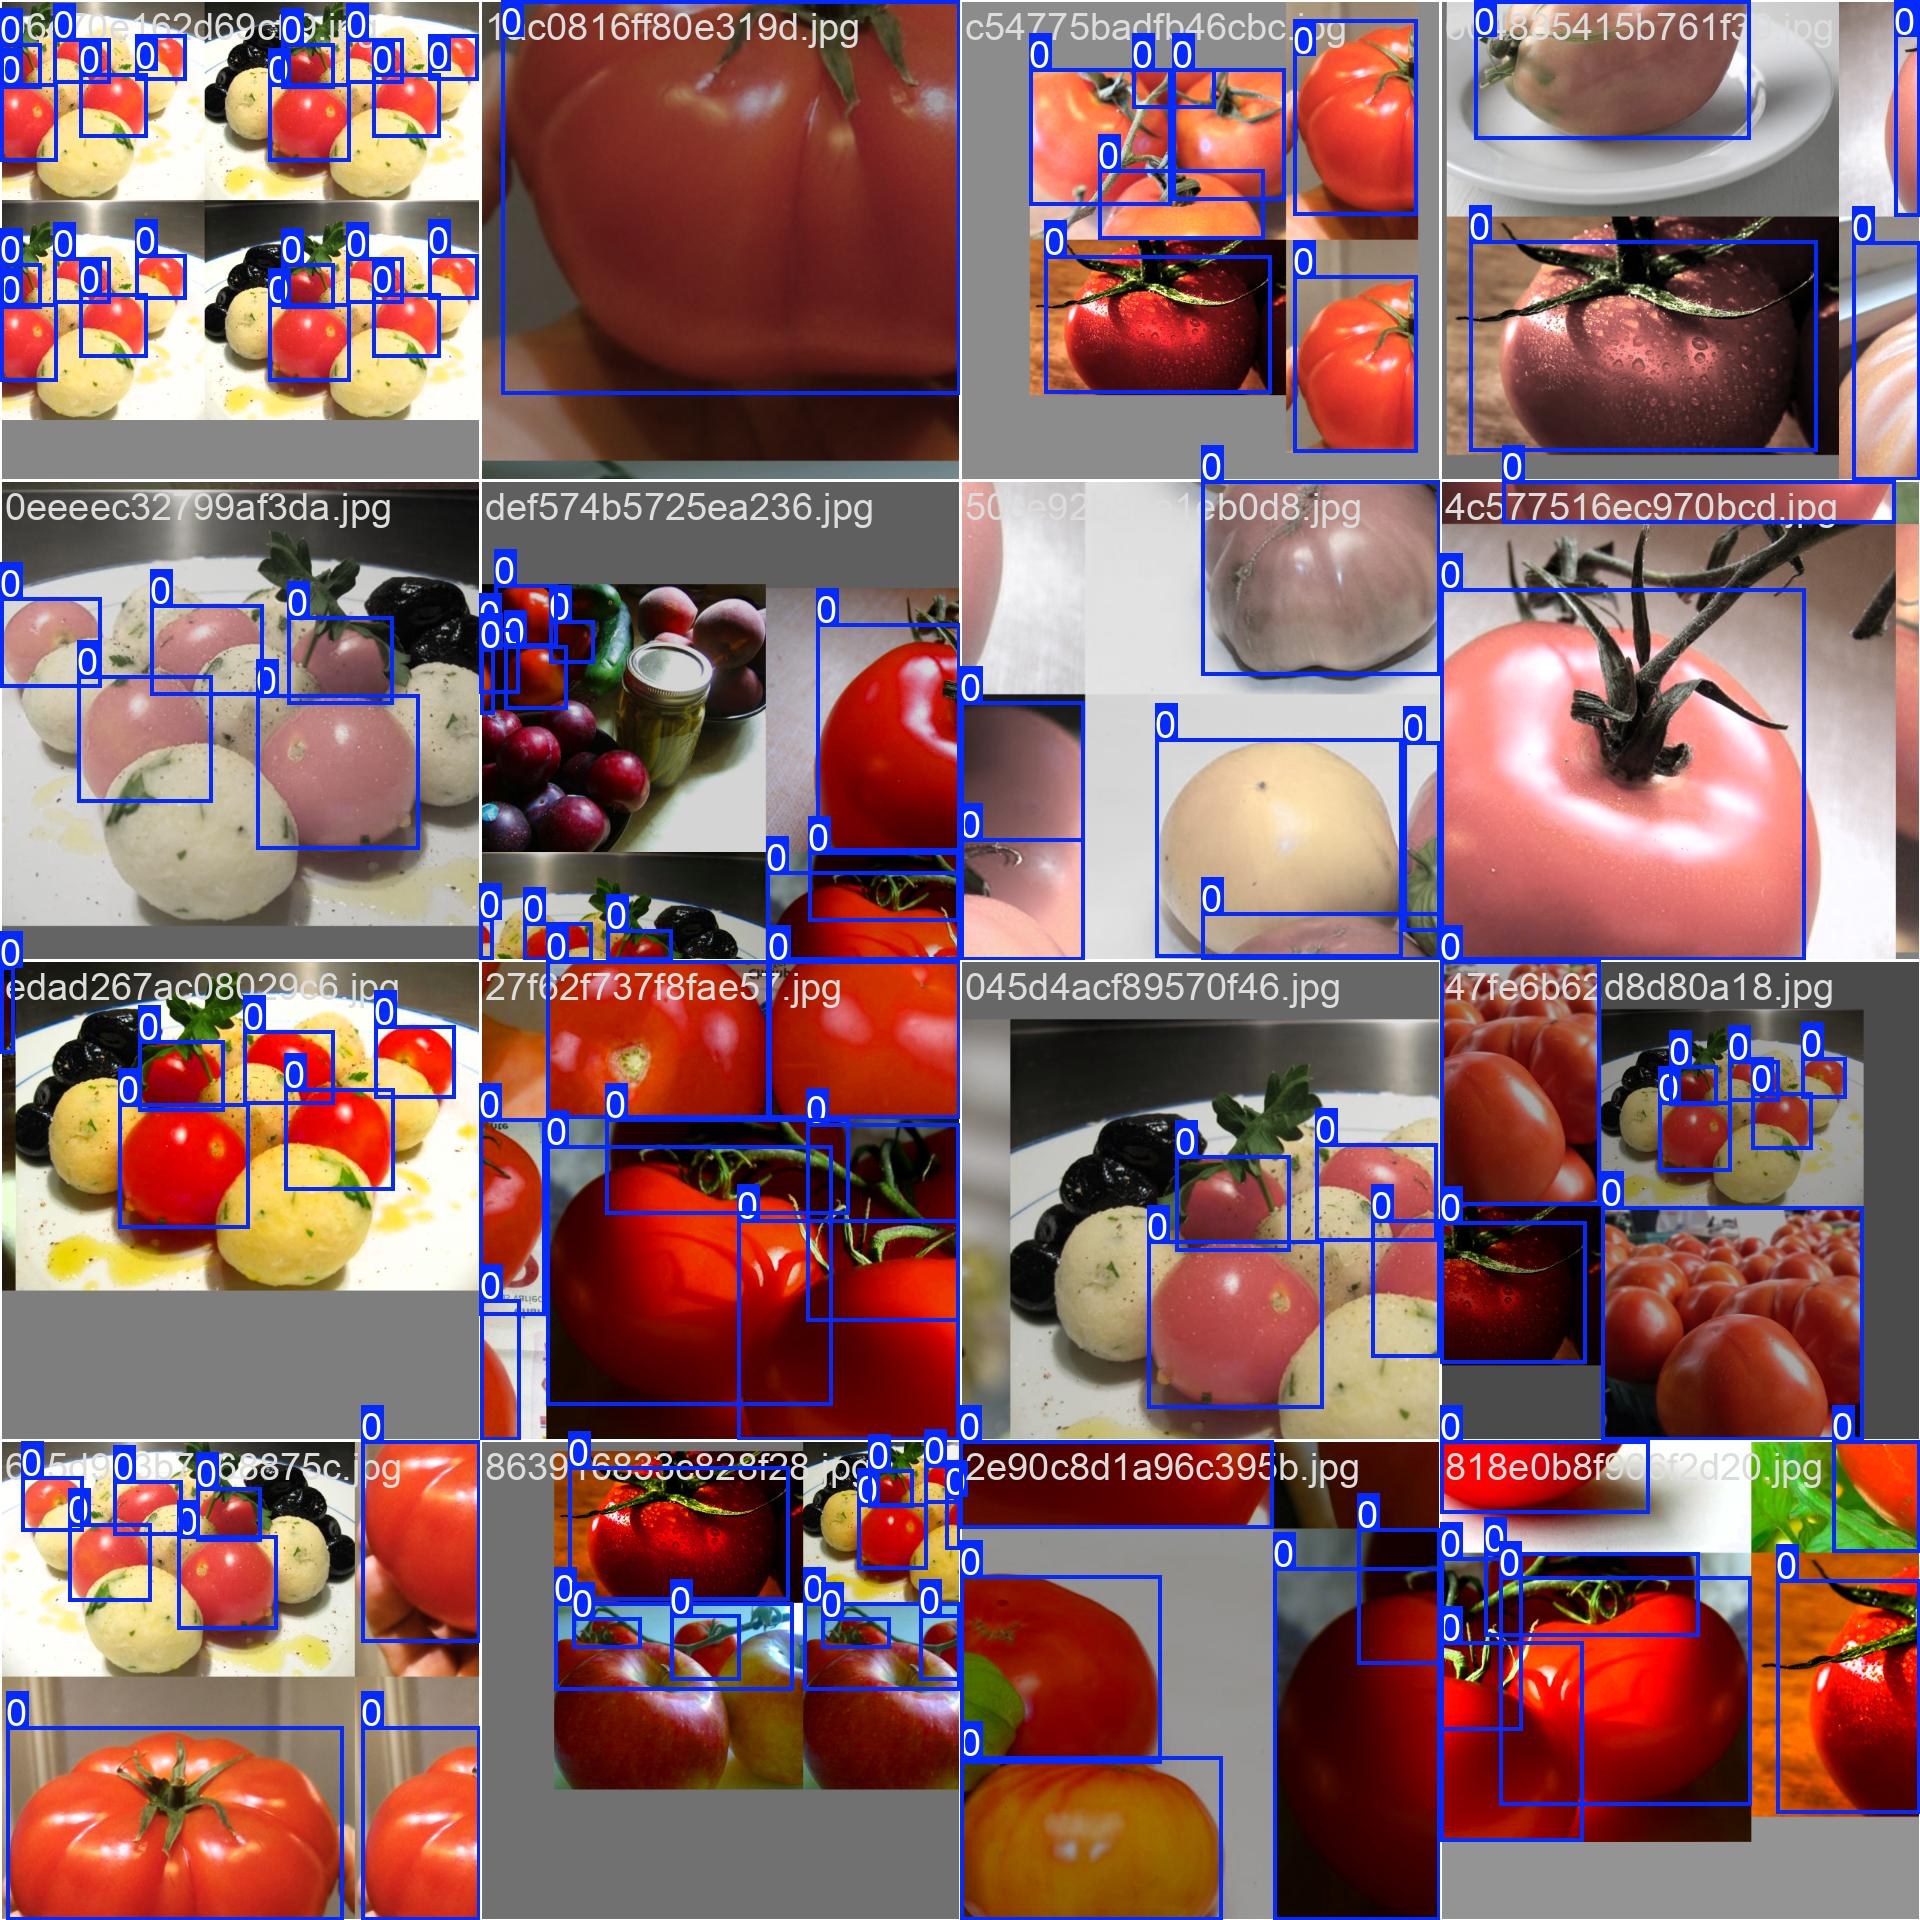
\includegraphics[width=0.42\textwidth]{figures/dataset_train_batch.jpg}
\caption{A training batch after Ultralytics augmentation (mosaic, flips, color jitter). Green boxes are ground-truth labels from Open Images.}
\label{fig:batch}
\end{figure}

\subsection{Training and Results}

I followed the assigned Roboflow Colab. Since my dataset does not live on the Roboflow platform, I replaced the download cell with a direct upload of \texttt{dataset.zip}. I changed three training arguments and kept the rest at their defaults:

\begin{itemize}
  \item \texttt{model=yolo11n.pt} instead of \texttt{yolo11s.pt}, to match Experiment 1;
  \item \texttt{data} pointed at my \texttt{data.yaml} (one class, \texttt{tomato});
  \item \texttt{epochs=150} instead of 10, because a 42-image training set needs many passes, and an earlier 50-epoch run produced correct boxes with confidence scores that were too low to survive standard thresholds.
\end{itemize}

Training took about five minutes on the T4. The best checkpoint reaches precision 0.788, recall 0.714, mAP50 0.727, and mAP50-95 0.607 on the 8-image validation set. The validation set is small, so I read these numbers as indicative rather than precise. Figure~\ref{fig:curves} shows the training curves, and Figure~\ref{fig:cm} shows the confusion matrix: 12 of 21 ground-truth tomatoes are detected, 9 are missed, and 3 background regions are falsely detected.

\begin{figure}[h]
\centering
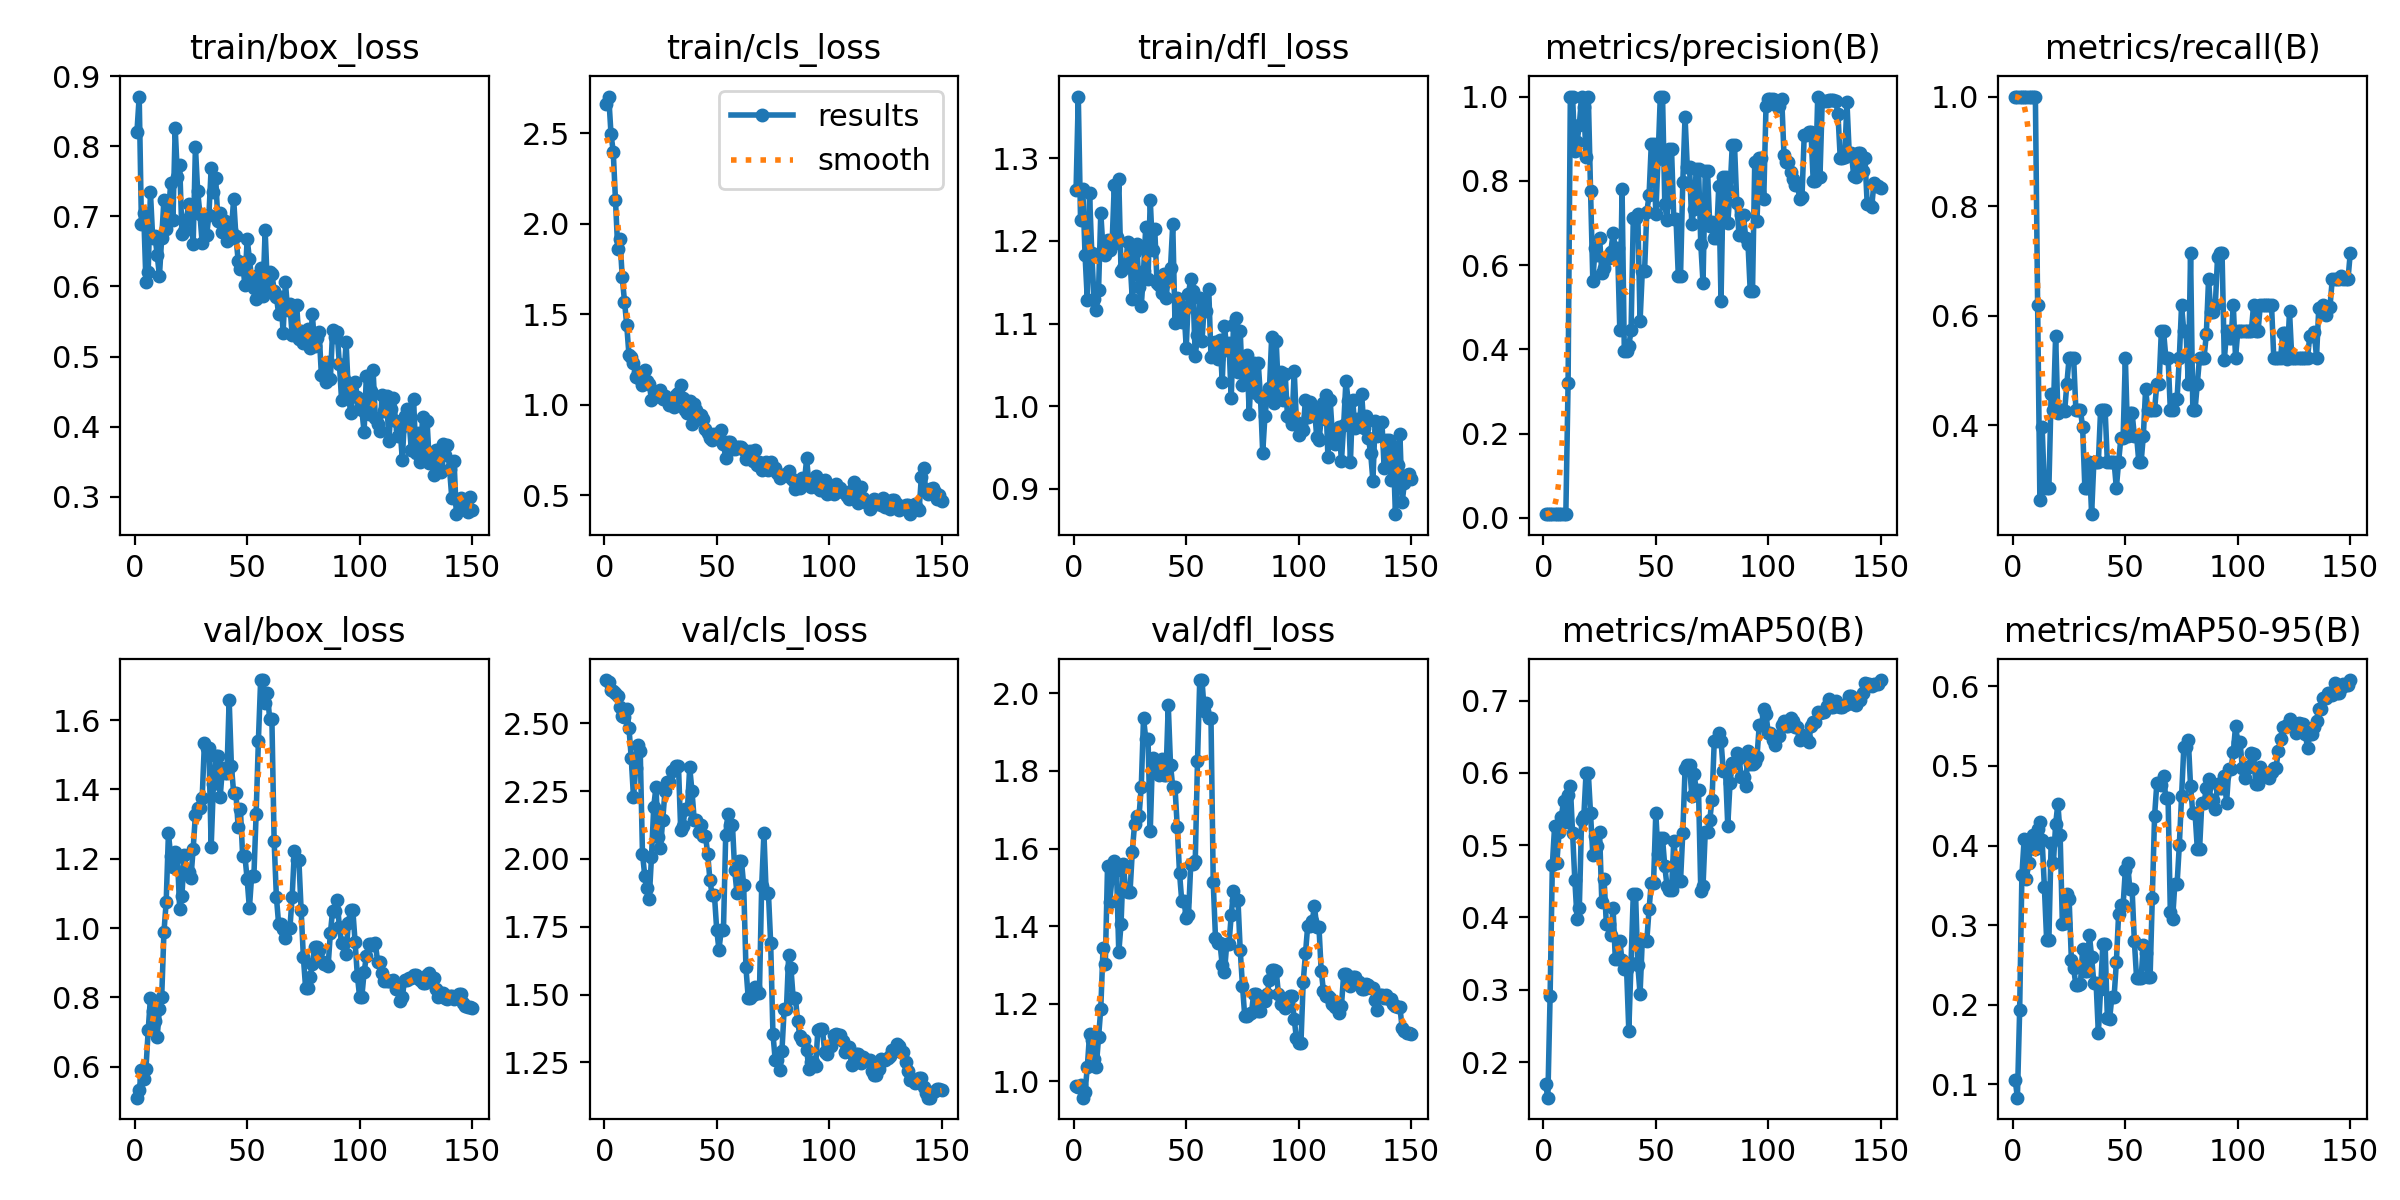
\includegraphics[width=0.68\textwidth]{figures/training_curves.png}
\caption{Training losses (left three columns, train on top and validation below) and validation metrics (right two columns) over 150 epochs.}
\label{fig:curves}
\end{figure}

\begin{figure}[h]
\centering
\begin{subfigure}{0.4\textwidth}
  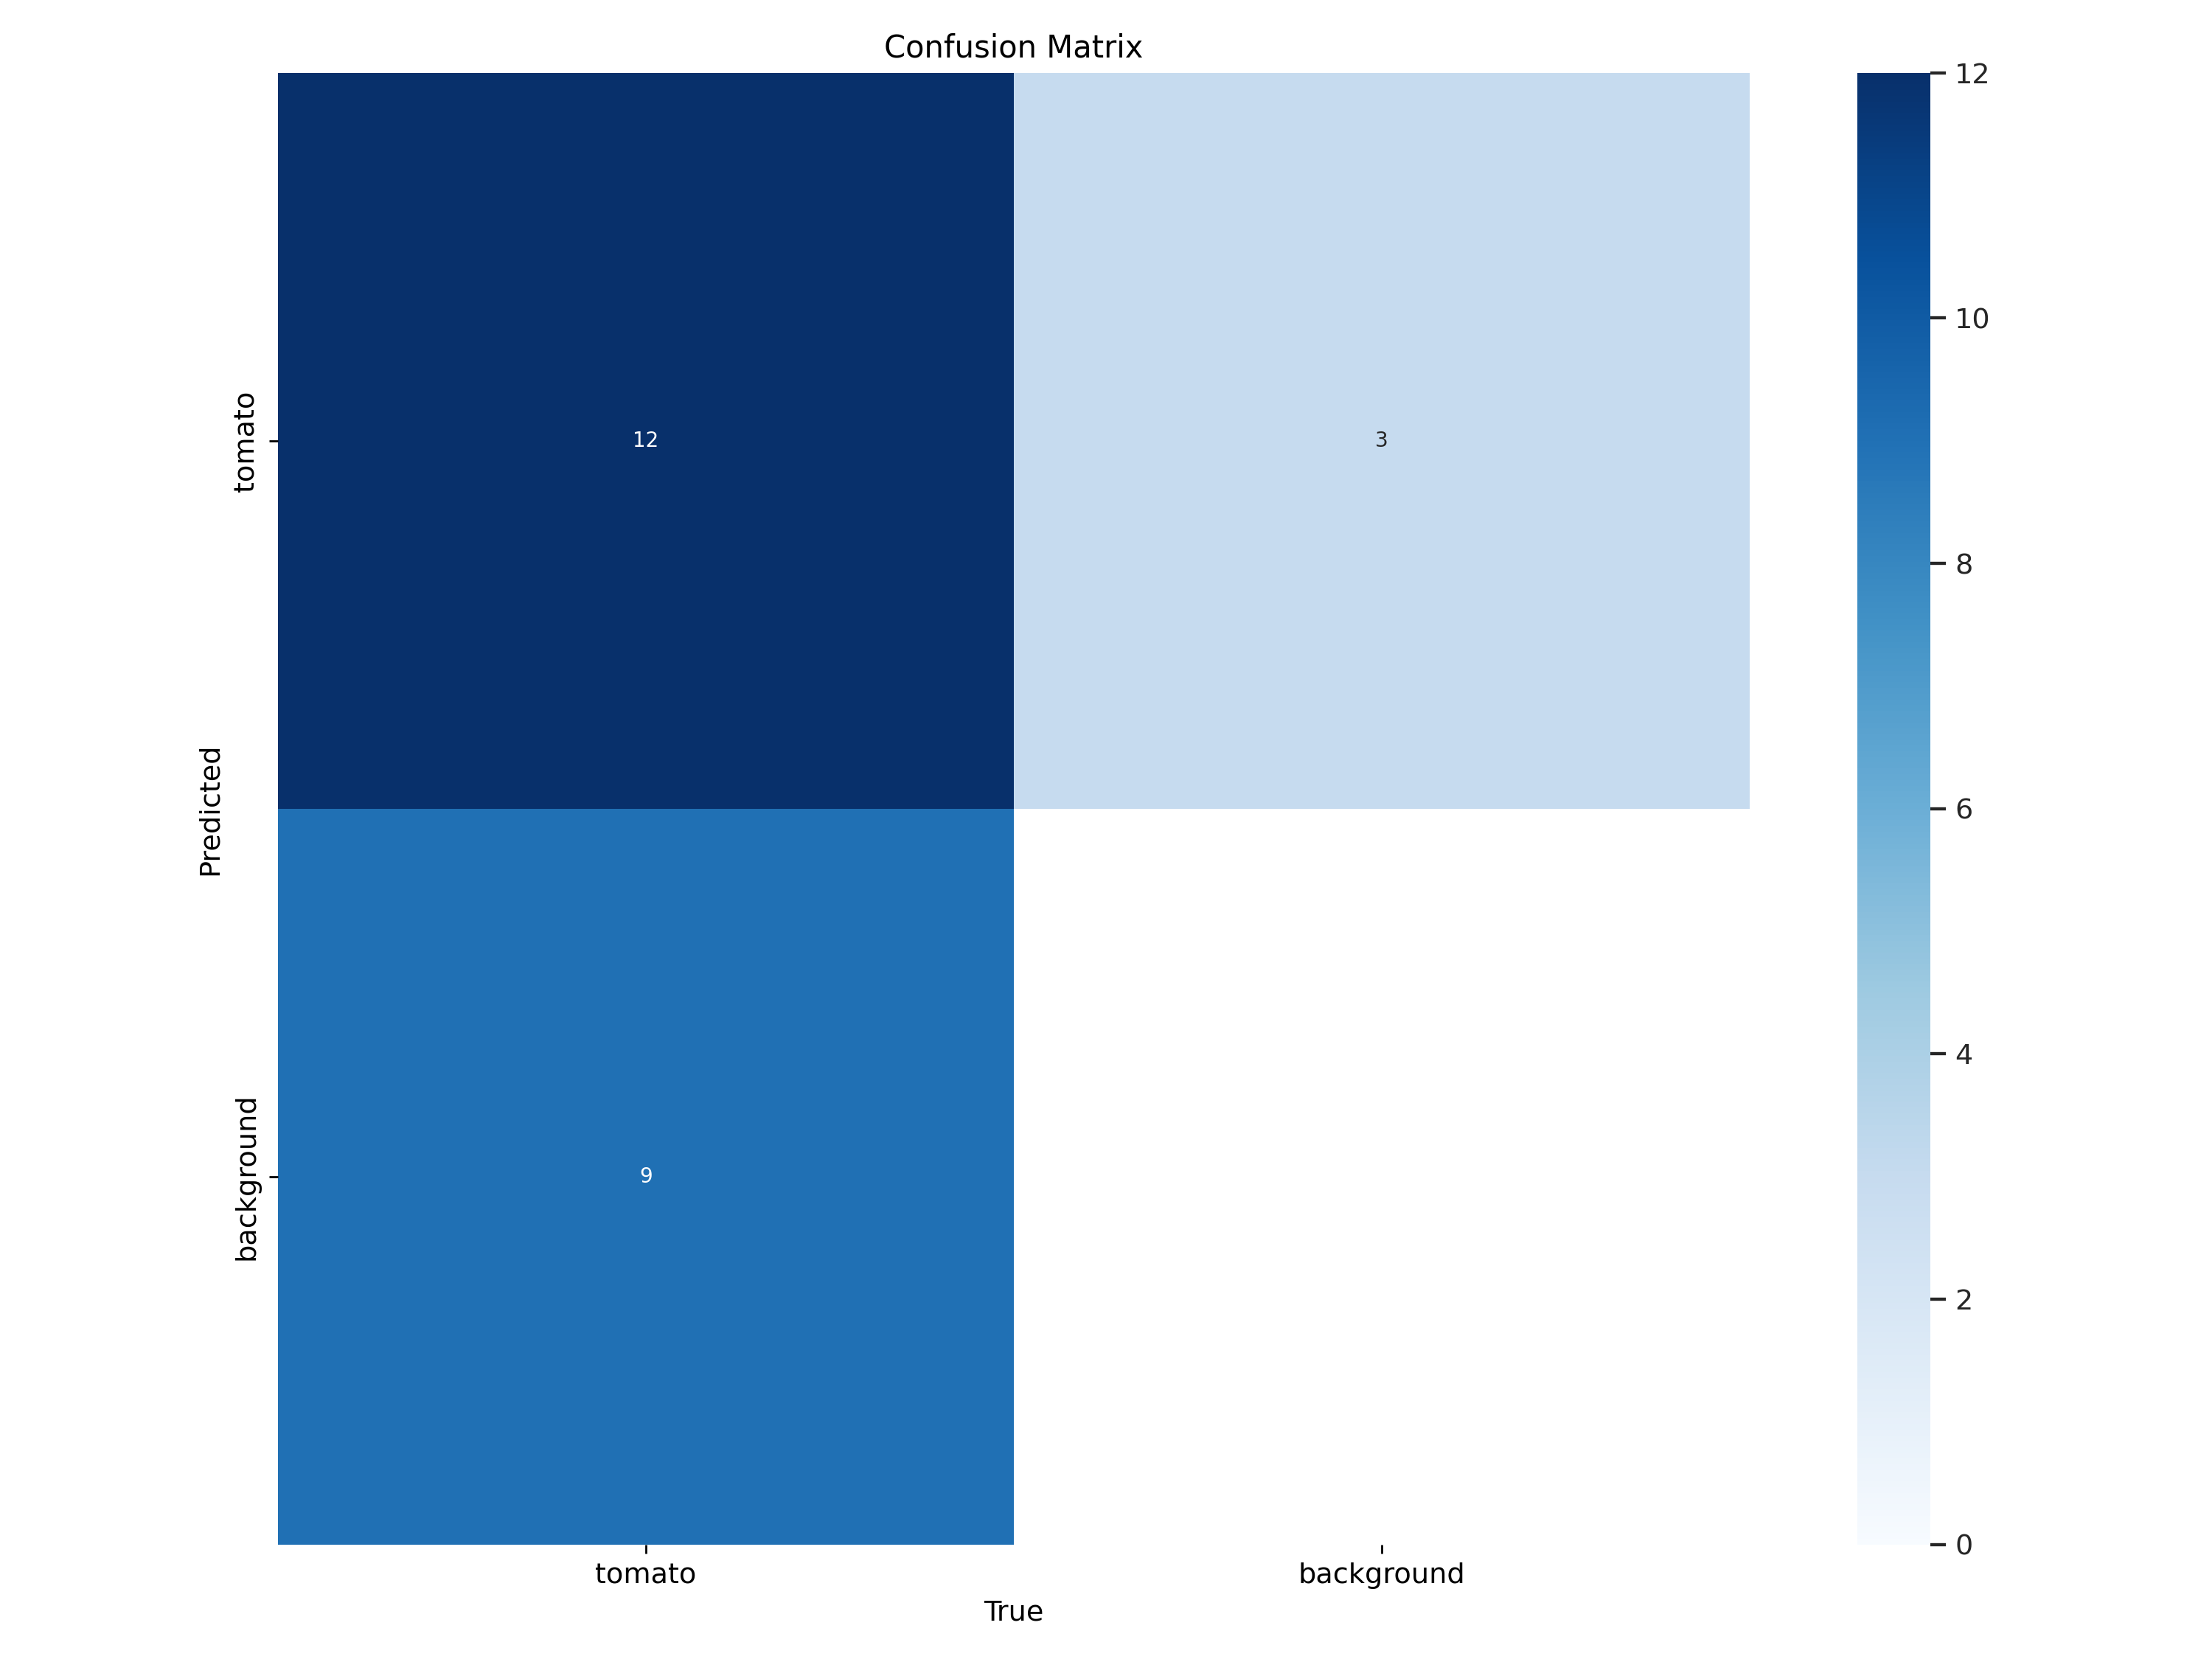
\includegraphics[width=\textwidth]{figures/confusion_matrix.png}
  \caption{Confusion matrix at a 0.25 threshold.}
  \label{fig:cm}
\end{subfigure}
\hfill
\begin{subfigure}{0.46\textwidth}
  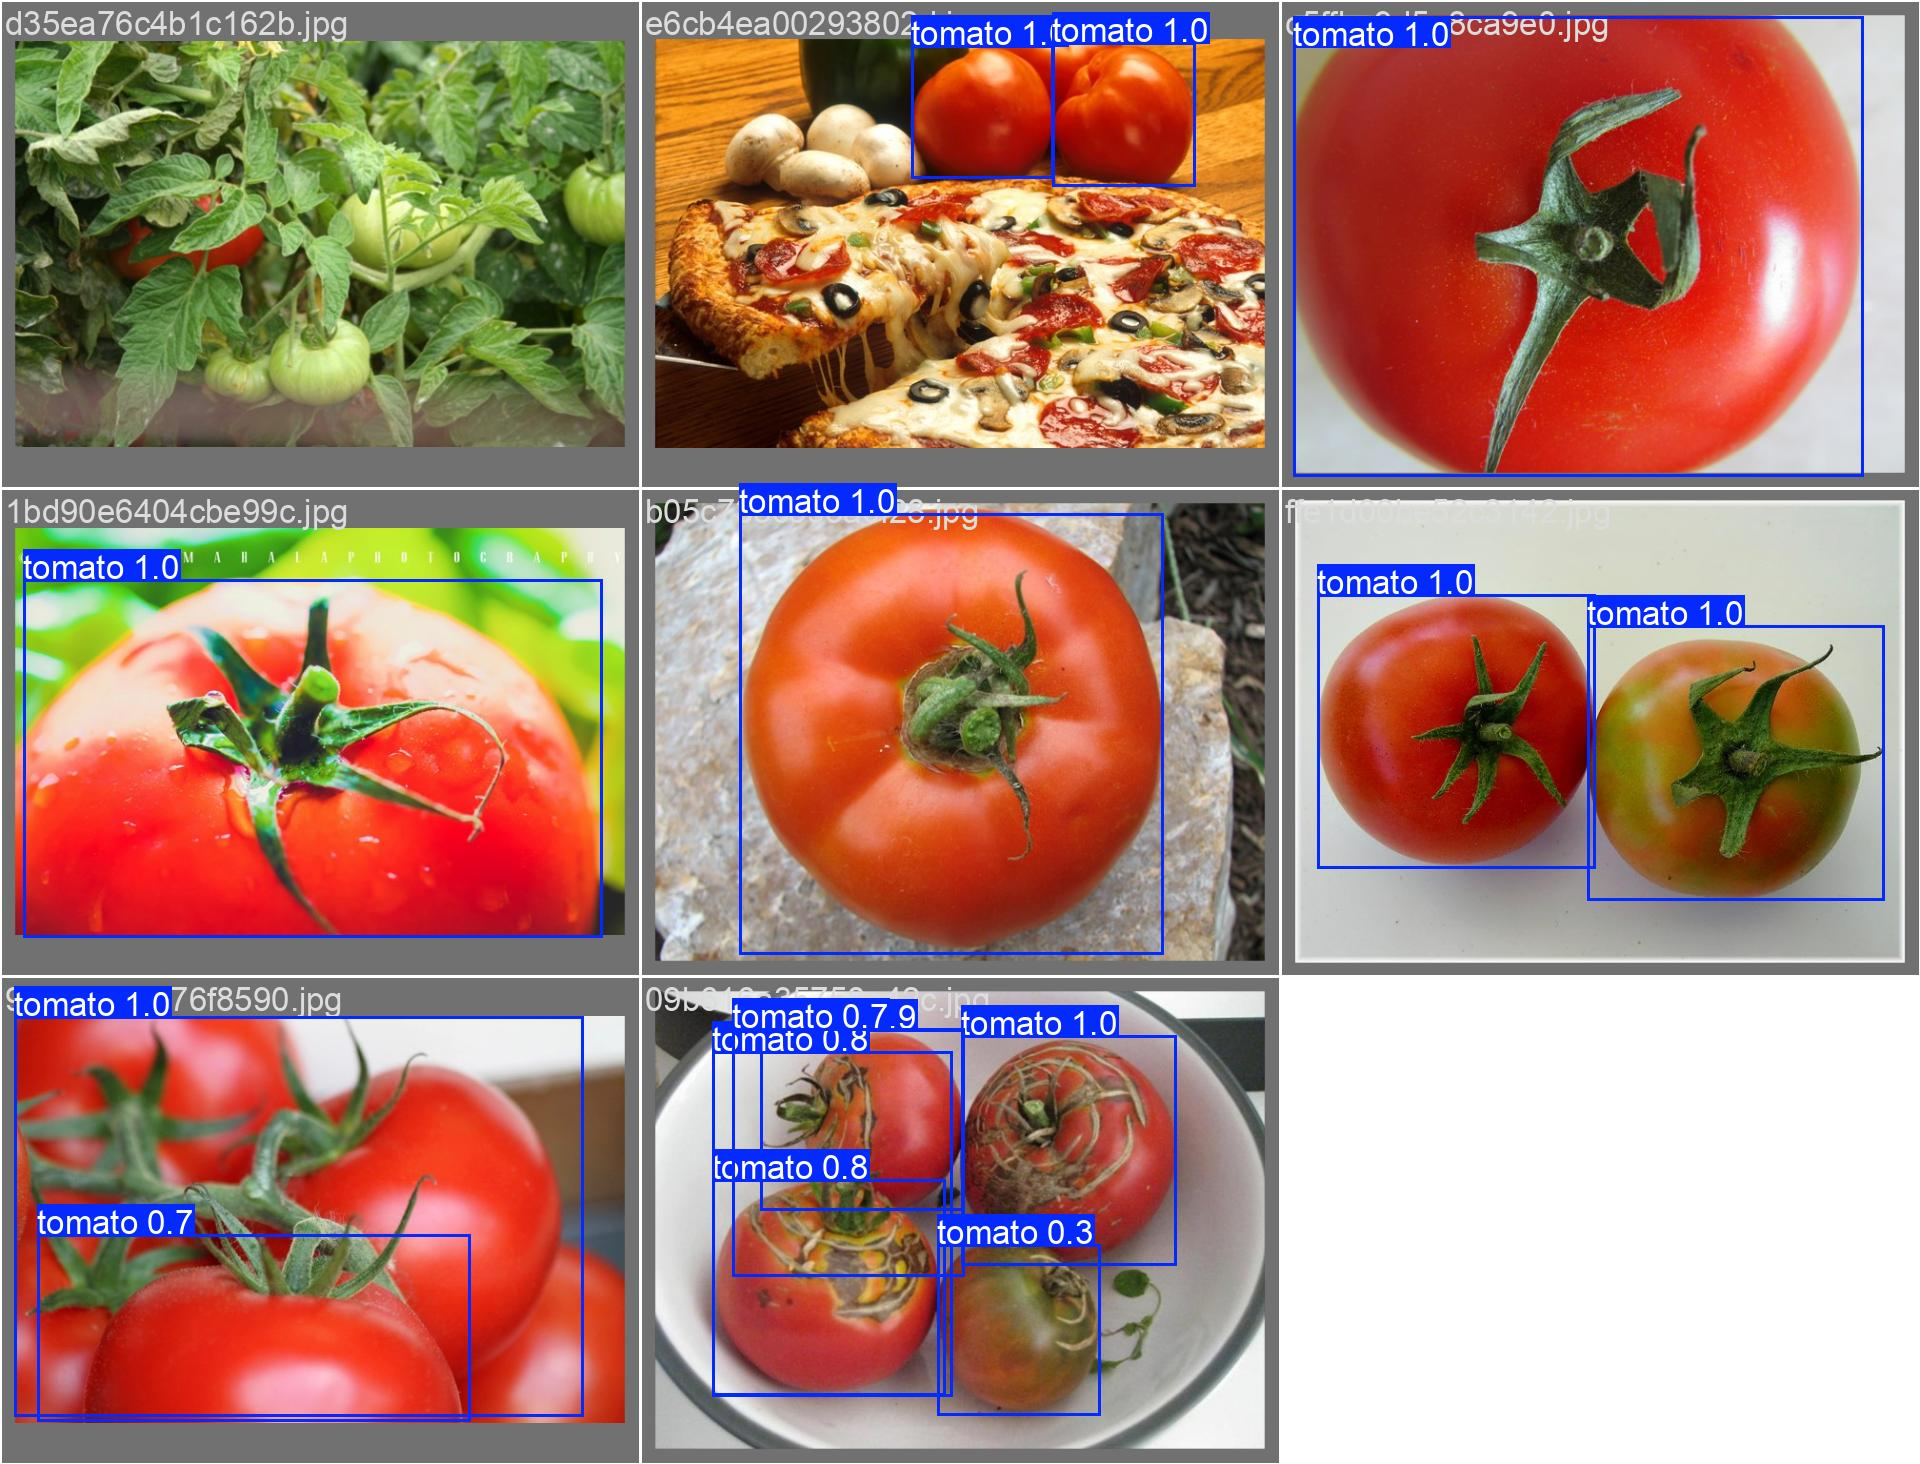
\includegraphics[width=\textwidth]{figures/val_predictions.jpg}
  \caption{Predictions on the validation images.}
\end{subfigure}
\caption{Fine-tuned model behavior on the validation set.}
\label{fig:valpred}
\end{figure}

\subsection{Repeating Experiment 1}

I exported \texttt{best.pt}, loaded it in the same webcam script, and held the same vine tomatoes in front of the camera. The pretrained model had labeled them \texttt{apple} at 0.62. The fine-tuned model labels the cluster \texttt{tomato} at 0.96 (Figure~\ref{fig:after}). Holding the toilet paper roll produces no detection, which is expected: the fine-tuned model only knows the single class it was trained on, and it lost the 80 COCO classes in the process.

\begin{figure}[h]
\centering
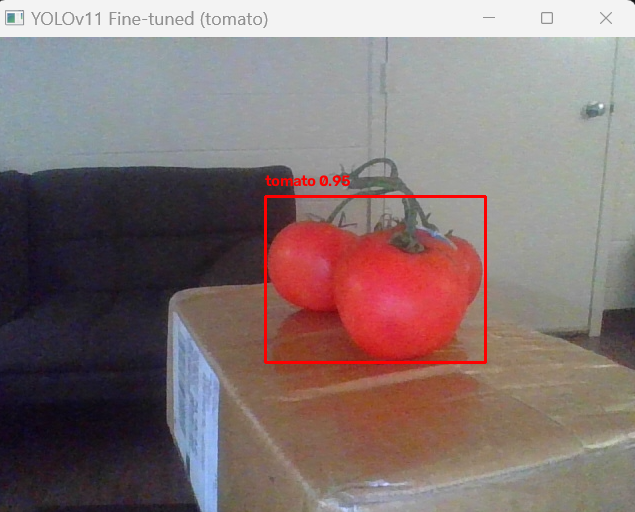
\includegraphics[width=0.38\textwidth]{figures/after_tomato_cluster.png}
\caption{The same tomatoes after fine-tuning: \texttt{tomato}, 0.96.}
\label{fig:after}
\end{figure}

\subsection{What I Learned from Fine-Tuning}

Fine-tuning helps, and the comparison above shows it directly. Four lessons stand out to me.

First, data quality mattered more than data quantity in my runs. Fifty noisy images trained a model that scored reasonably on mAP yet detected nothing at practical thresholds. Fifty curated images fixed the problem without any change to the training recipe.

Second, per-class data volume sets a floor. The toilet-paper class failed with about 12 training images, while tomato succeeded with 42. Transfer learning from COCO features lowers the data requirement, but it does not remove it.

Third, metrics need to be read together with an operating threshold. My intermediate models looked acceptable on mAP, which integrates over all thresholds, while the confusion matrix at 0.25 showed zero detections. Both views were true; only their combination told me what a deployed model would actually do.

Fourth, fine-tuning on a narrow class list causes forgetting. The specialized model no longer detects bottles or couches. For a product that needs both old and new classes, I would either include the old classes in the fine-tuning data or keep two models.

\section{Experiment 3: Open-Set Detection with YOLOE}

\subsection{What Open-Set Object Detection Is}

A closed-set detector can only assign labels from the class list fixed at training time. My two models illustrate the limitation from both sides: pretrained YOLOv11n forced every unknown object into one of 80 COCO classes, and my fine-tuned model knows exactly one word. Open-set (open-vocabulary) detection removes the fixed list. The user supplies a prompt at inference time, either as text (class names such as ``tomato'') or as a visual example (a reference box), and the detector localizes objects that match the prompt, including categories it was never explicitly trained on.

I followed the assigned YOLOE Colab. With the text prompt \texttt{["dog", "eye", "nose", "tongue"]}, the model detected all four concepts on the example image, including object parts that no COCO-style detector would output (Figure~\ref{fig:yoloe}). The visual-prompt section of the notebook repeats the idea with a drawn reference box instead of words.

\begin{figure}[h]
\centering
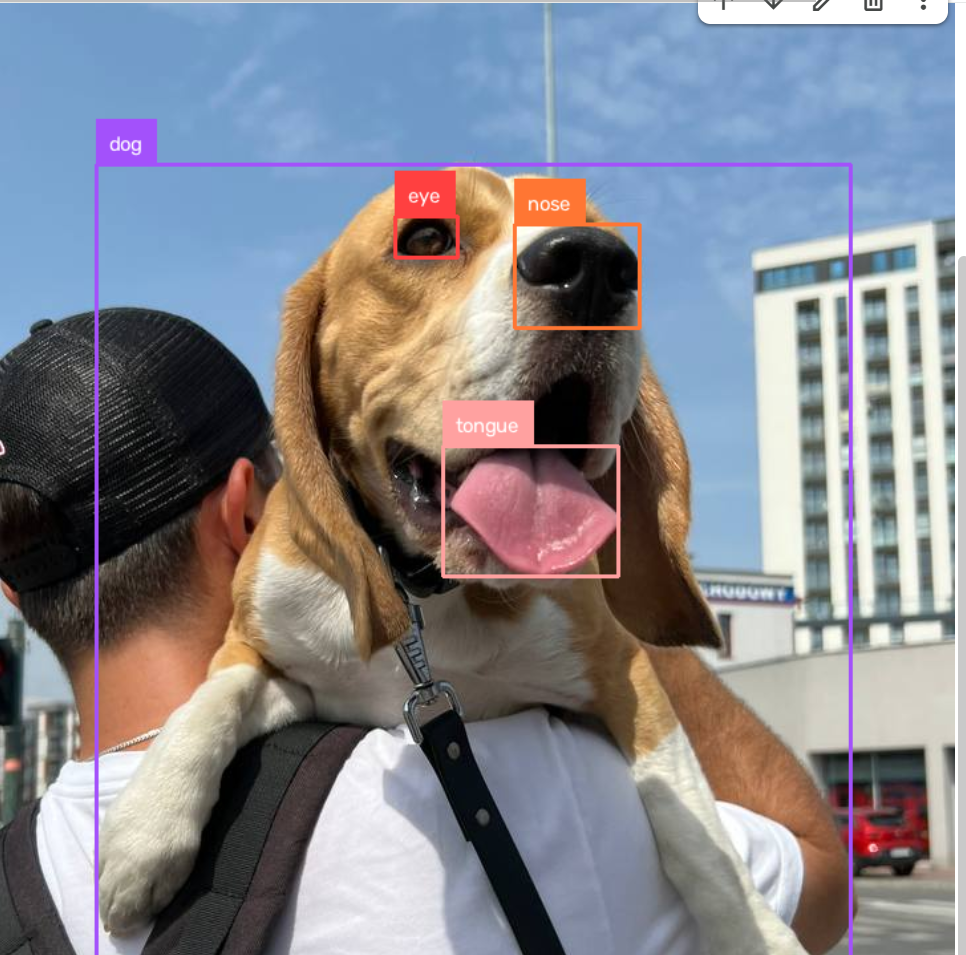
\includegraphics[width=0.36\textwidth]{figures/yoloe_text_prompt.png}
\caption{YOLOE text-prompt detection: dog, eye, nose, and tongue, with no training on these prompts.}
\label{fig:yoloe}
\end{figure}

\subsection{YOLOE Architecture and What Makes Open-Set Possible}

YOLOE keeps the familiar YOLO skeleton. The backbone follows YOLOv8/YOLOv11 design, and the neck is a standard PAN that fuses the P3, P4, and P5 scales. Speed therefore stays in the real-time range. The decisive change sits in the head. A closed-set YOLO head ends in a classification layer whose weight rows are fixed class prototypes, one row per training class. YOLOE replaces that layer with an anchor-free, decoupled head whose classification branch outputs an \emph{embedding} and scores each region by similarity against prompt embeddings. The class list becomes an input rather than a trained parameter.

Three prompt encoders produce those embeddings. RepRTA handles text prompts: class names pass through a CLIP-style text encoder once, and the resulting vectors act as the classification weights. SAVPE handles visual prompts by encoding a reference box into the same space. LRPC covers the prompt-free mode with a built-in vocabulary of about 4{,}585 classes. During large-scale pretraining on region-text data, the detector learns to place each region's embedding close to the text embedding of its label, so at inference time a new word lands in a meaningful position of the shared space and matching still works.

Two consequences are worth noting. A plain COCO-trained YOLO checkpoint cannot be reused directly, because its region features were never aligned with a text space; the alignment pretraining is what open-set capability costs. In the other direction, once a vocabulary is fixed, the prompt embeddings fold back into an ordinary classification layer through re-parameterization, so a deployed YOLOE pays no runtime overhead. The contrast with Experiment 2 summarizes the trade-off: teaching my closed-set model one new word took a curated 50-image dataset and 150 epochs, while YOLOE handled unseen words from a single line of text, using a larger model and an expensive pretraining stage paid once by its authors.

\section{Conclusion}

The three experiments form one arc. A pretrained closed-set detector works well inside its 80 classes and fails predictably outside them. Fine-tuning extends the class list at the cost of data collection, training, and forgetting; my iterations suggest that curation quality and per-class volume decide whether the result is usable. Open-set detection moves the class decision from training time to inference time, which removes the retraining cost for new categories.

\section*{AI Use Statement}

Per the course AI policy, I disclose that I used Claude (Anthropic) as an assistant throughout the lab: for environment setup and debugging, for building and curating the Open Images dataset, for step-by-step guidance through the Colab notebooks, and for drafting and revising the text of this report. I ran all experiments myself and take responsibility for all content, code, and results.

\end{document}
